\documentclass[tikz]{standalone}

% \usepackage{newtxtext,newtxmath}

%!TEX root = main.tex

% mytikzset
\usepackage{tikz}
\usetikzlibrary{positioning,arrows,shapes,patterns}
\usetikzlibrary{decorations.pathmorphing}
\usetikzlibrary{decorations.markings}
\usetikzlibrary{decorations.pathreplacing}
\usetikzlibrary{calc}
\usetikzlibrary{patterns}
\usetikzlibrary{decorations.markings}
\usetikzlibrary{petri}

\tikzset{
  vector/.style={thick,double,draw=black, postaction={decorate},
    decoration={markings,mark=at position .6 with {\arrow[black,scale=0.4]{triangle 45}}}},
  axial/.style={thick,double,densely dashed,draw=black, postaction={decorate},
    decoration={markings,mark=at position .6 with {\arrow[black,scale=0.4]{triangle 45}}}},
  gluon/.style={decorate, draw=black,
    decoration={coil,aspect=0.3,segment length=5pt,amplitude=3pt}},
  pseudo/.style={thick, dashed, draw=black, postaction={decorate},
    decoration={markings,mark=at position .6 with {\arrow[red,scale=0.5]{triangle 45}}}},
  scalar/.style={thick,draw=black, postaction={decorate},
    decoration={markings,mark=at position .6 with {\arrow[black,scale=0.5]{triangle 45}}}},
  cut/.style={draw=black, decorate, decoration={snake, segment length=1mm, amplitude=0.2mm}}
}

\definecolor{myGreen}{RGB}{0,127,0}

\begin{document}
\nopagecolor
  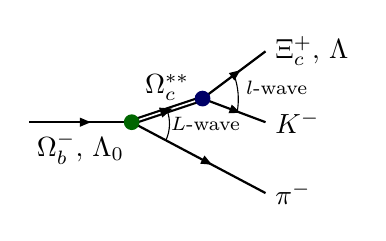
\begin{tikzpicture}[node distance=0.9cm and 1.3cm, baseline=1cm]
    \coordinate[] (c0);
    \coordinate[{left}=of c0] (Lamc);
    \coordinate[above right=of c0, xshift=-4mm, yshift=-6mm] (c1);
    \coordinate[above right=of c0, xshift=4mm, label=right:{$\Xi_c^+,\,\Lambda$}] (p);
    \coordinate[      right=of c0, xshift=4mm, label=right:{$K^-$}] (K);
    \coordinate[below right=of c0, xshift=4mm, label=right:{$\pi^-$}] (pi);

    \draw[] ($(c0)!0.5!(c1)$) arc(20:-24:0.5) node[yshift=2mm, xshift=5mm] {\scriptsize$L$-wave};

    \draw[] ($(c1)!0.5!(p)$) arc(20:-10:0.9) node[yshift=3mm, xshift=5mm] {\scriptsize$l$-wave};

    \draw[scalar]  (Lamc) -- node[below] {$\Omega_b^-,\,\Lambda_0$} (c0);
    \draw[vector]  (c0) -- node[above] {$\Omega_c^{**}$} (c1);
    \draw[scalar]  (c1) -- (p);
    \draw[scalar]  (c1) -- (K);
    \draw[scalar]  (c0) -- (pi);

    \fill[green!40!black] (c0) circle (1mm);
    \fill[blue!40!black] (c1) circle (1mm);
  \end{tikzpicture}
\end{document}
